\begin{refsection}
\chapter{Introduction}

The importance of non-bonding interactions in our world simply cannot be overstated.
While we may think of the more familiar covalent and ionic bonds as the core of chemistry, more often than not it is non-bonding interactions that dictate the nature of substances, from bulk properties such as tensile strength, to microscopic phenomena like protein-ligand interactions.

At a fundamental level, all non-bonding interactions (indeed, conventional bonding too) are attributable to the electrostatic force.
However, it is more convenient to broadly categorise interactions based on strength and structural motifs that are common to each class.
Such classes include dispersion forces, dipole-dipole interactions, and hydrogen bonding (H-bonding).
In the 19th century, it became apparent that these classes paint an incomplete picture of intermolecular bonding.
As part of their investigation into solvent effects on the colour of iodine solutions in 1949, Bensei and Hildebrand invoked the concept of ``charge-transfer'' complexes to explain the association of molecular iodine with nucleophilic solvent molecules.\autocite{Benesi1949}
Although the electrophilic nature of molecular halogens was already well appreciated with respect to reactivity, this appears to be the first acknowledgement that this understanding could be applied to ground state complexes.
In support of this, Hassel and Hvoslef elucidated the structure of a 1:1 complex of molecular bromine and 1,4-dioxane in 1954, and observed an unusually strong interaction between the two molecules.\autocite{Hassel1954}
The crystal was comprised of long chains of monomers (\cref{fig:hassel-xray}), exhibiting a very short \ce{O \cdots Br} contact (2.71~\AA, the sum of the van der Waals (VDW) radii is 3.37~\AA), and a slightly lengthened \ce{Br-Br} bond (2.31~\AA\ vs 2.28~\AA\ in gaseous bromine).

\begin{figure}[ht]
  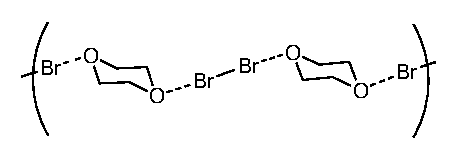
\includegraphics[width=0.6\columnwidth]{Figures/hassel-xray.eps}
  \caption[Bromine-dioxane complex.]{Long chains of molecular bromine and 1,4-dioxane, observed by Hassel and Hvoslef.}\label{fig:hassel-xray}
\end{figure}

In the subsequent years, a wide variety of names and labels were applied to the ``charge-transfer'' phenomenon, including ``lock and key'', ``donor-acceptor'', and ``filling of anti-bonding orbitals'', as summarised in Bent's excellent 1968 review\autocite{Bent1968}.
The term ``halogen bonding'' (X-bonding) only gained widespread acceptance in 1983 after the review of Dumas, Gomel, and Guerin.\autocite{Dumas1983}
The term deliberately evokes similarity to the better known concept of hydrogen bonding, as the two phenomena are of comparable strength and, importantly, directionality.
In 1998 Anthony C. Legon again used the term to describe the attractive interaction between halogens and Lewis bases in pre-reactive complexes, harking back to the original understanding of electrophilic halogens as a primarily reactive phenomenon.\autocite{Legon1998,Legon1999}
In the following years, the potential of X-bonding was more fully recognised, with applications in supramolecular chemistry and self-assembly\autocite{Corradi2000,Metrangolo2008,Priimagi2013}, catalysis and bond activation\autocite{Walter2011,Soloshonok2017,Takagi2017}, and molecular sensing and recognition\autocite{Cornes2017,VargasJentzsch2013,Borissov2017}.

From X-bonding grew the related concepts of chalcogen (Ch-), pnictogen (Pn-), and tetrel bonding (T-bonding), as the electrophilic nature of these elements was discovered.\autocite{Murray2007}
Similar applications have also been found for these classes of non-covalent interactions, Ch-bonding in particular.\autocite{Fanfrlik2014,Garrett2016,Ho2016,Wonner2017,Mitchell2017,Benz2017,Biot2018,Ho2017}

\section{Chalcogen Bonding}
Ch-bonding is the attractive interaction between a Lewis base and a chalcogen atom bearing an electron withdrawing substituent (\cref{fig:ch-bonding-intro}).
The terminology of Ch-bonding partners is perhaps counter-intuitive, as donors and acceptors are named by analogy with H-bonded equivalents.
Note this is contrary to the formal flow of electron density; Ch-bond \emph{donors} bear vacant \emph{acceptor} orbitals, while Ch-bond \emph{acceptors} are \emph{donors} of electron density.
For the purposes of this thesis, ``donor'' will refer to the Lewis acidic chalcogen species.

\begin{figure}
    \centering
    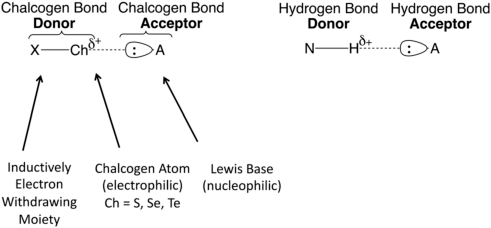
\includegraphics[width=0.8\linewidth]{Figures/ch-bonding.pdf}
    \caption{Chalcogen bonding model, and similarity to H-bonding.}\label{fig:ch-bonding-intro}
\end{figure}

\subsection{Mechanisms}
As was discussed in the previous section, all intermolecular (and indeed \emph{intra}mole\-cular) forces are manifestations of the electromagnetic force.
Nonetheless, it is more convenient to categorise energetic contributions to any given interaction as orbital, electrostatic, or dispersion mediated, as there are marked differences in strength and directionality between them.
Historically, X- and Ch-bond interactions were understood to be primarily due to orbital overlap and resulting charge transfer.
Evidence for this included the lengthening of the \ce{X-X} bond corresponding to increased occupation of the $\sigma^{\star}$(\ce{X-X}) orbital due to the incoming lone pair (this was observed in Hassel and Hvoslef's original work\autocite{Hassel1954}).
Characteristic charge transfer bands are also observed in the UV-vis spectra of halogen solutions.\autocite{Blackstock1987}

Such evidence of orbital contributions is not, however, common to all systems displaying X- or Ch-bond interactions.
The iodoperfluoroalkanes and arenes studied by \citeauthor{Yan2014} show no charge transfer bands in UV-vis spectra, yet are exceptionally strong X-bond donors.\autocite{Yan2014}
Jane Murray and Peter Politzer have advocated for an alternative, primarily electrostatic explanation of X- and Ch-bond interactions.\autocite{Murray2008,Murray2009}
They propose that a positively charged $ \sigma $-hole is generated along the extension of a $ \sigma $ bond to an electron withdrawing substituent, due to polarisation of the electron cloud.
This also adequately explains the strength and directionality of these interactions.
An interpretation which has not attracted as much attention is that of dispersion forces.

While the varying contributions from each of these factors can be dissected computationally via perturbation methods, experimental evidence is surprisingly sparse.
Pascoe, Ling and Cockroft, however, devised an elegant experiment to quantitatively determine energetic contributions.\autocite{Pascoe2017}
\textsuperscript{19}F NMR was used to determine the relative populations of two conformers of a ``molecular balance'', one bearing a Ch-bond interaction, one not (\cref{fig:cockroft-balances}).
Interaction energies were thus derived, and found to be more or less invariant with respect to the solvent.
This appeared to rule out electrostatic contributions, as solvent dipole moment and bulk polarisability would otherwise have a large effect on the position of the equilibrium.
These results also suggest that dispersion plays only a minor role, for similar reasons.

\begin{figure}
    \centering
    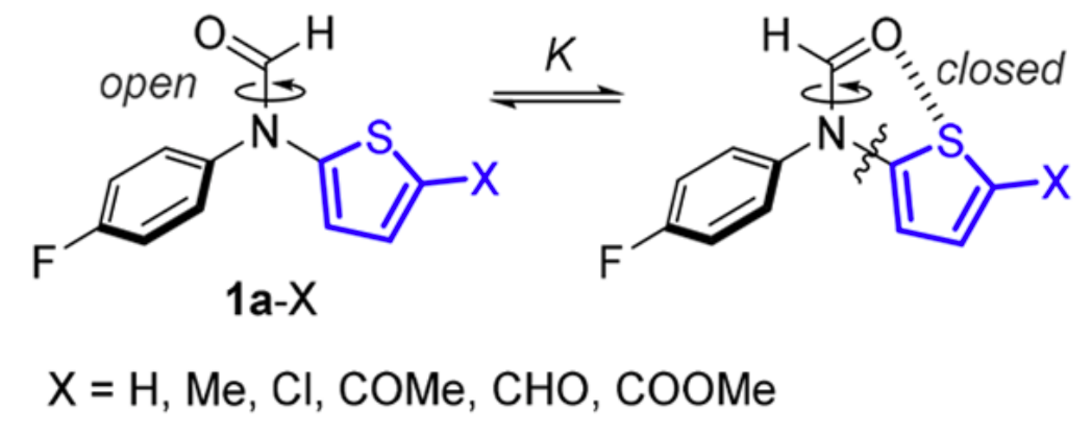
\includegraphics[width=0.6\linewidth]{Figures/cockroft-balances.pdf}
    \caption{``Molecular balances'' designed by \citeauthor{Pascoe2017} for the measurement of Ch-bond energies.\autocite{Pascoe2017}}\label{fig:cockroft-balances}
\end{figure}

DFT was used to further probe the dispersion contribution.
Free energies were calculated using functionals which both did, and did not include dispersion corrections, and the values compared to the experimental results.
The non-dispersion corrected B3LYP functional gave superior correlation with experiment than did either M06-2X and $ \omega $B97-D, both of which include dispersion.
This provided additional evidence that, in the systems studied, the major contributor to the interaction is orbital overlap and charge transfer.

Although current evidence points towards these interactions being primarily orbital related, the electrostatic ``$ \sigma $-hole'' terminology of Politzer and Murray has stuck, and the term is now used to encompass the whole gamut of X-, Ch-, Pn-, and T-bonding interactions.

\section{Applications of Ch-Bonding}
Ch-bonding, and by extension, all $ \sigma $-hole interactions can theoretically be applied to any formal Lewis acid-base system.
They are especially attractive as a hydro\emph{phobic} complement to H-bonding interactions, which are generally considered to be hydro\emph{philic}.
The following are brief summaries of existing applications in the literature.

\subsection{Materials}
The major applications of $ \sigma $-hole interactions have so far been in the realm of crystal engineering.
Early work by \citeauthor{Corradi2000} showed that halogen bonding was able to outcompete H-bonding in the formation of supramolecular architectures.\autocite{Corradi2000}
A review by \citeauthor{Metrangolo2008} summarised the forms that are accessible using X-bonding to direct crystal growth.\autocite{Metrangolo2008}
1D, 2D, and 3D architectures are able to be generated using appropriate X-bond donors, and these show potential in the design of liquid crystals, organic semiconductors and paramagnetic materials (\cref{fig:iodotempo-chains})
A more recent review by the same group described applications in anion transport, and luminescent and photo-responsive crystals.\autocite{Priimagi2013}
The group of Stefan Matile has further explored anion transport, and has published a review comparing X-bonding with other hydrophobic interactions such as anion-$ \pi $ and anion-macrodipole interactions (\cref{fig:matile-anion-binder}).\autocite{VargasJentzsch2013}

\begin{figure}
    \centering
    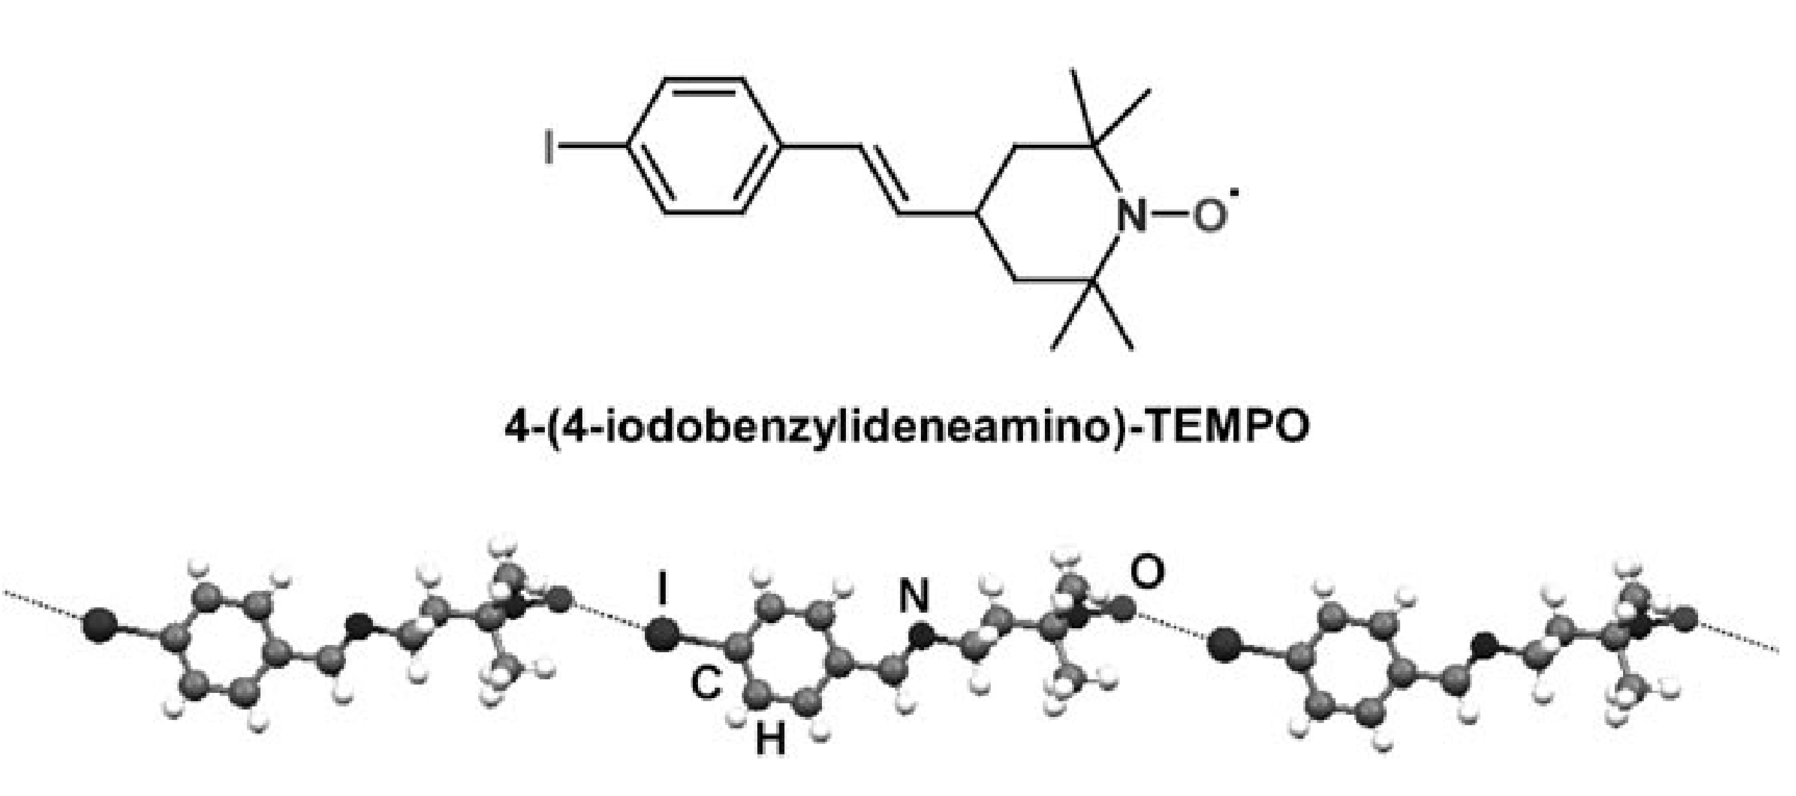
\includegraphics[width=0.6\linewidth]{Figures/iodotempo-chains.pdf}
    \caption{One-dimensional chains of 4-(4-iodobenzylidene)-TEMPO structured by X-bonds.\autocite{Metrangolo2008}}\label{fig:iodotempo-chains}
\end{figure}

\begin{figure}
    \centering
    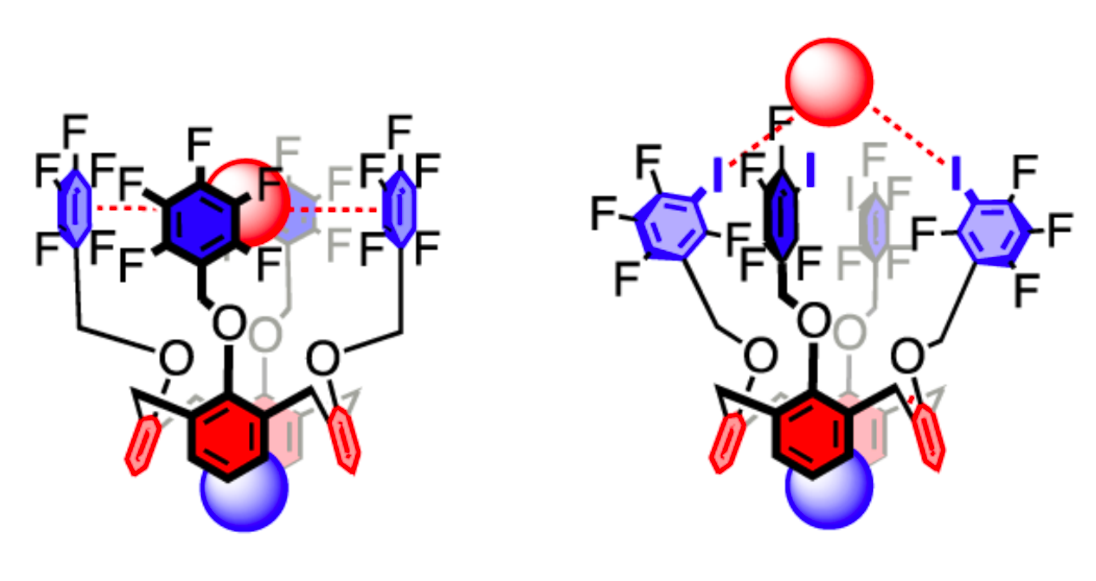
\includegraphics[width=0.4\linewidth]{Figures/matile-anion-binder.pdf}
    \caption{Anion binding through anion-$ \pi $ interactions and X-bonding.\autocite{VargasJentzsch2013}}\label{fig:matile-anion-binder}
\end{figure}

Ch-bonding, too, has been investigated with respect to materials chemistry.
\citeauthor{Fanfrlik2014} demonstrated the importance of Ch-bonding on the crystal packing of thiaboranes.\autocite{Fanfrlik2014}
They found that the sulfur-based $ \sigma $-hole was sufficiently strong to interact with the weakly basic $ \pi $ electrons of a phenyl group, with contacts as short as 3.2~\AA\ being observed (\cref{fig:thiaborane-ch-bond}).

\begin{figure}
    \centering
    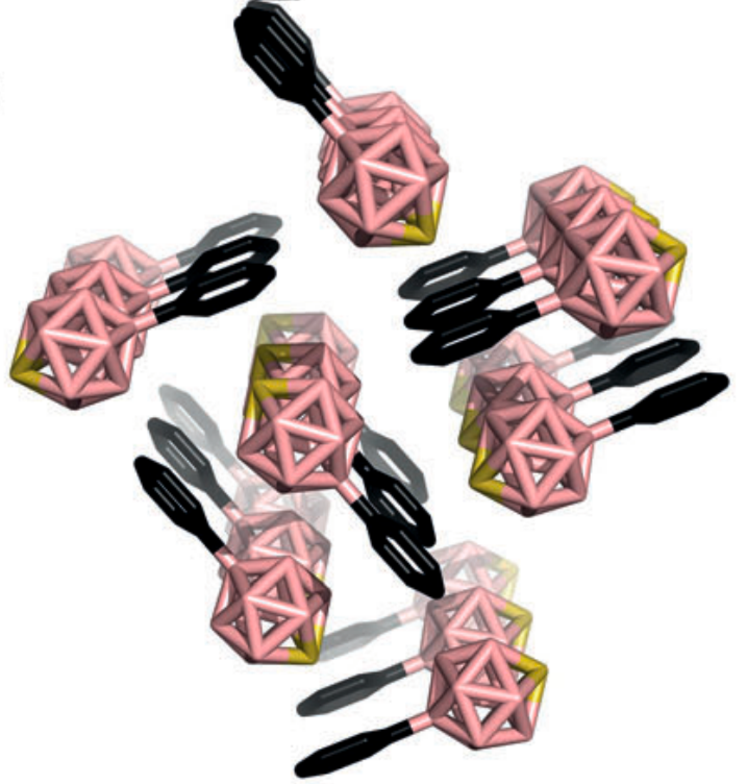
\includegraphics[width=0.45\linewidth]{Figures/thiaborane-ch-bond.pdf}
    \caption{Ch-bonding in thiaboranes.\autocite{Fanfrlik2014}}\label{fig:thiaborane-ch-bond}
\end{figure}

In 2016, \citeauthor{Ho2016} published their work into tellurium-based Ch-bonding.\autocite{Ho2016}
Their scaffolds are based on an iso-tellurazole N-oxide, which reversibly forms macrocyclic structures that persist in both gas and solution phase (\cref{fig:te-pd-macrocycle}).
The macrocycles were found to coordinate \ce{Pd2+}.
This is particularly interesting, as the tellurium atoms are simultaneously behaving as a Lewis acid and base.
The authors point out that such soft macrocycles are quite rare, and their work could facilitate further studies of transition metals in a soft coordination environment.
They went on to investigate benzo-fused derivatives of iso-tellurazoles, as well as selenium analogues, which crystallised to form macromolecular pores and voids.\autocite{Ho2017}

\begin{figure}
    \centering
    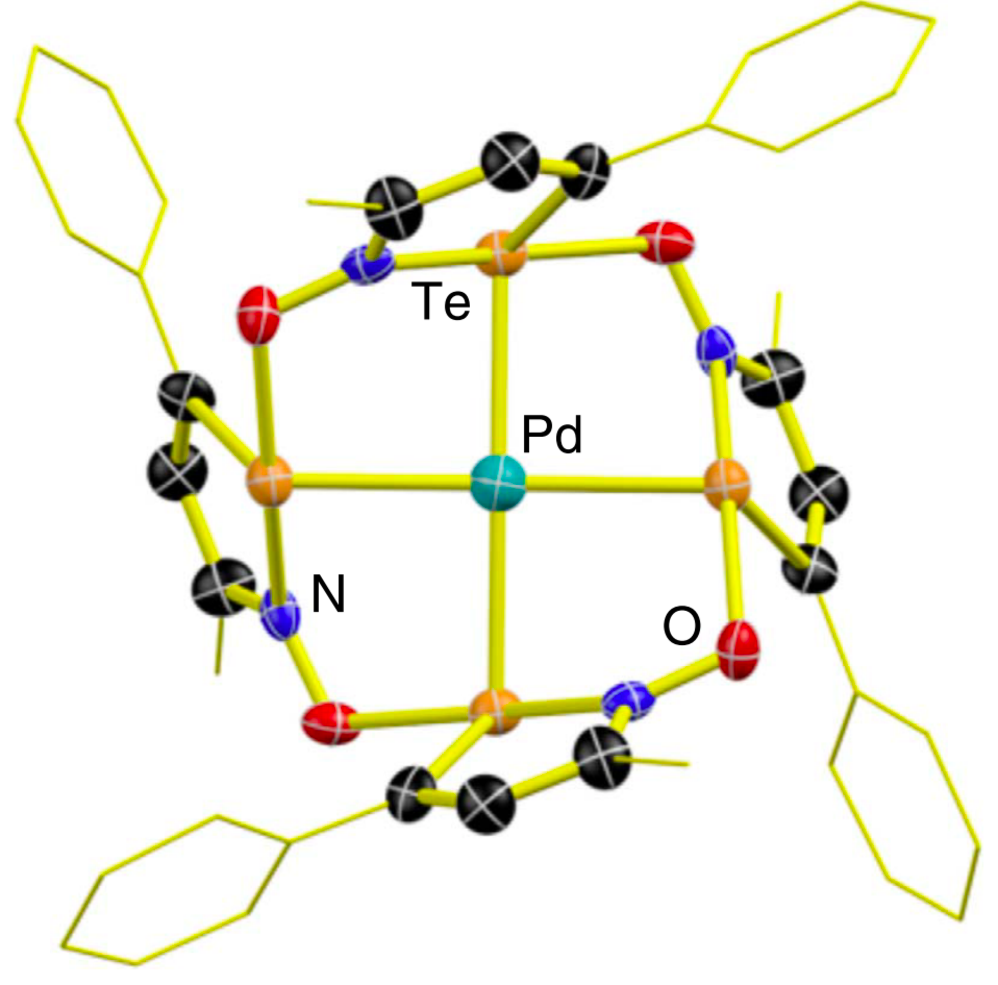
\includegraphics[width=0.4\linewidth]{Figures/te-pd-macrocycle.pdf}
    \caption{A tetrameric macrocycle held together by Ch-bonds.\autocite{Ho2016}}\label{fig:te-pd-macrocycle}
\end{figure}

The Taylor group has been active in the development of X- and Ch-bonding molecular sensors.
Early work demonstrated that X-bonding tridentate ligands (reminiscent of enterobactin) showed moderate selectivity for \ce{Cl-}.\autocite{Dimitrijevic2010}
They later developed bidentate Ch-bonding ligands which exhibited a tenfold increase in association constant with respect to chloride (\cref{fig:taylor-cl-binder}).\autocite{Garrett2015a,Garrett2016}

\begin{figure}
    \centering
    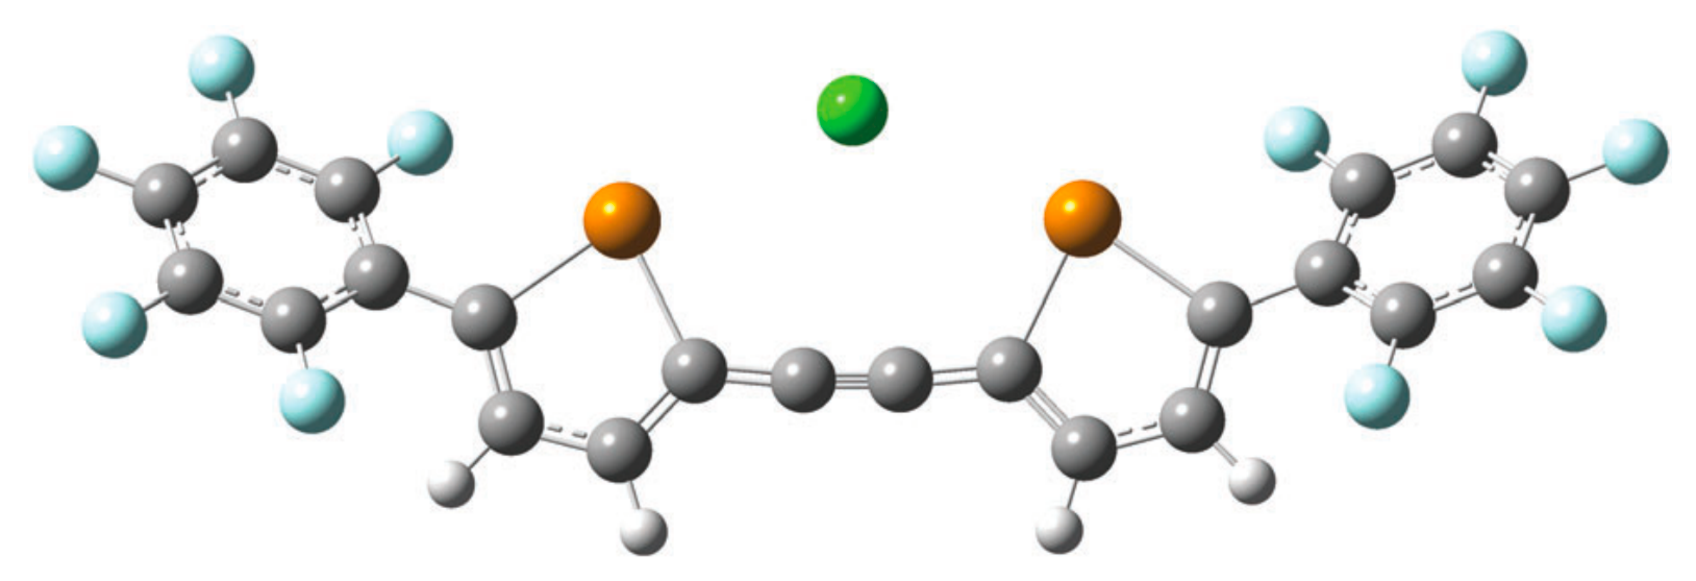
\includegraphics[width=0.6\linewidth]{Figures/taylor-cl-binder.pdf}
    \caption{A bidentate Ch-bonding anion binder.\autocite{Garrett2016}}\label{fig:taylor-cl-binder}
\end{figure}

Similar results have been achieved by the Beer group, who have developed X-bonding sensors for the perrhenate anion.\autocite{Cornes2017}
These sensors are based on functionalised cyclodextrins, and are even more sensitive than the corresponding H-bonding analogues.
The group has also use iodotriazole scaffolds to chelate anions.\autocite{Borissov2017}
Incorporation of a chiral binaphthol moiety was shown to differentiate between enantiomers of chiral anions.

The role of selenium-based Ch-bonding on the crystal structure and mechanism of the drug ebselen was demonstrated by \citeauthor{Thomas2015}.\autocite{Thomas2015}
Ch-bonding between the selenium atom and carbonyl oxygen directs the crystal packing of this compound, and leads to the formation of one-dimensional chains of molecules (\cref{fig:ebs-packing}).
Interestingly, the Lewis acidity of the $ \sigma $-hole was invoked as an explanation of the antioxidant properties of the drug.

\begin{figure}
    \centering
    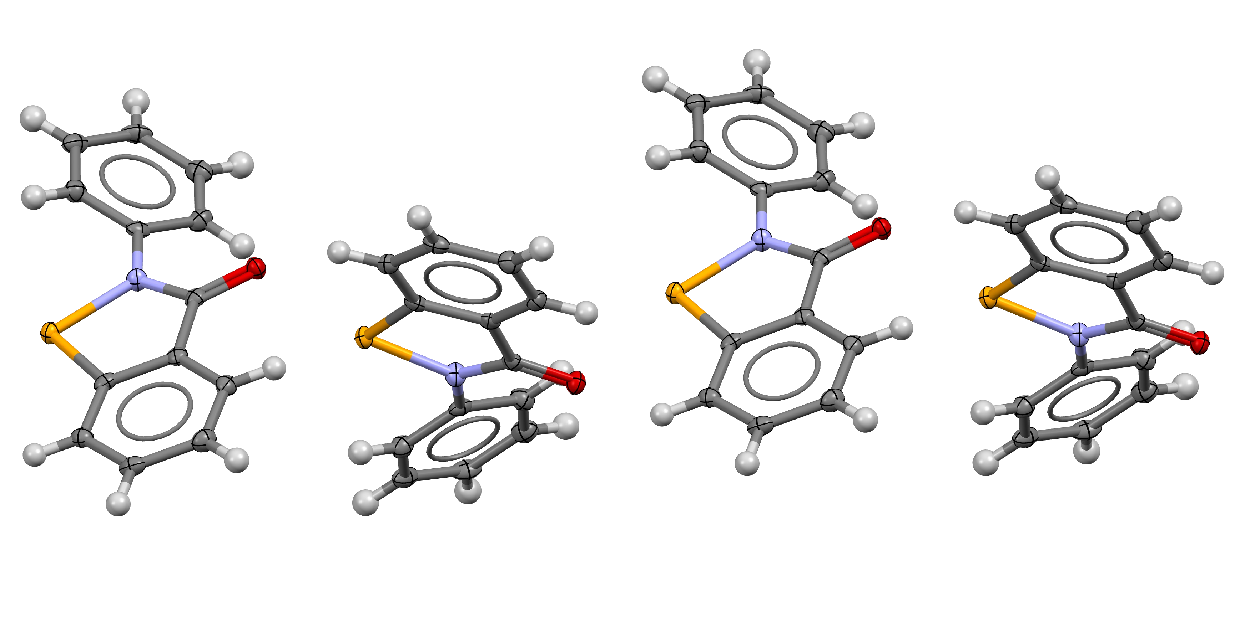
\includegraphics[width=0.7\linewidth]{Figures/ebs-packing.pdf}
    \caption{One dimensional chains formed in the crystal packing of ebselen.}\label{fig:ebs-packing}
\end{figure}

\subsection{Catalysis and bond activation}
In 2008, halogen bonding was first applied to a Hantzsch ester reduction of a quinoline derivative.\autocite{Bruckmann2008}
This reaction is well characterised and understood, and has been catalysed with a variety of Br\o nsted and Lewis acids.
The X-bond donors chosen were perfluoroiodoalkanes, and high conversions were achieved with modest catalyst loadings of 10\%.

In 2011, a modified Ritter reaction was devised wherein benzhydryl bromide was activated by a dicationic imidazolium-based X-bond donor to give the carbocation intermediate, which was then captured by acetonitrile and then hydrolysed to afford the amide product.\autocite{Walter2011}
This pioneering work was limited by the necessity of stoichiometric amounts of the X-bond donor, as it is consumed in the course of the reaction.

A similar alkylation of 1-chloroisochroman was achieved by the same group using a neutral perfluoroiodoarene X-bond donor in catalytic quantities.\autocite{Kniep2013}
The proposed mechanism is similar to the thiourea-catalysed reaction of \citeauthor{Reisman2008}\autocite{Reisman2008}, which has shown promise in asymmetric induction.
The authors noted issues with solubility of the perfluoroiodoarene catalysts, which is expected of such highly fluorinated compounds.

The reduction of quinoline was successfully catalysed by a dithiophene system by \citeauthor{Benz2017} in 2017\autocite{Benz2017}, and then again by the same group with a benzodiselenazole (\cref{fig:quinoline-redn}).\autocite{Benz2017a}
With the increased selectivity and strength of the Se-based Ch-bonding catalyst compared to the X-bonding perfluoroiodoalkane, the authors were able to reduce the catalyst loading to 1\%.

\begin{figure}
    \centering
    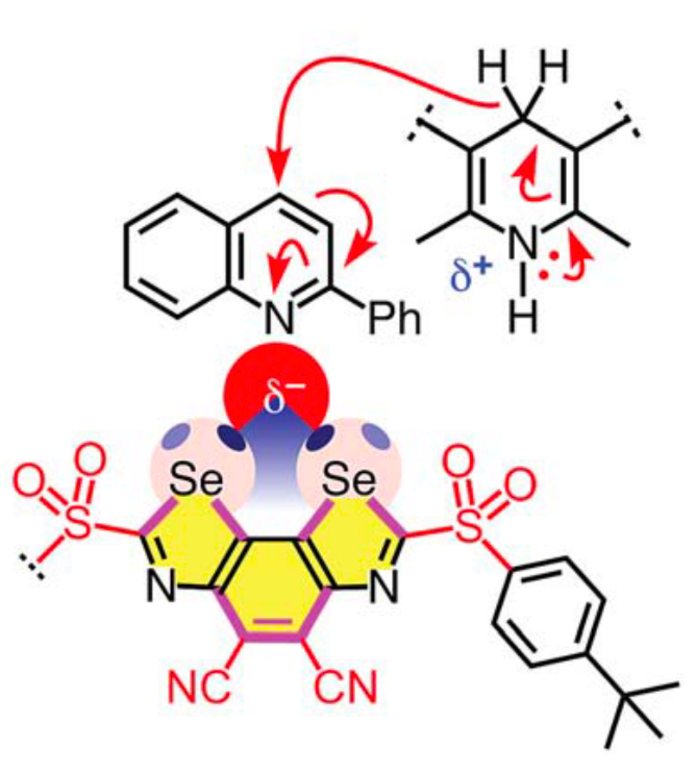
\includegraphics[width=0.4\linewidth]{Figures/quinoline-redn.pdf}
    \caption{Proposed mechanism for the catalytic reduction of quinoline by a Ch-bonding catalyst.\autocite{Benz2017}}\label{fig:quinoline-redn}
\end{figure}

\citeauthor{Wonner2017} developed a selenated bis-benzimidazolium Ch-bonding catalyst for the alkylation of 1-chloroisochroman, and solvolysis of benzhydryl bromide.\autocite{Wonner2017,Wonner2017a}
Although the best results were observed with the dicationic catalysts, conversion was also achieved with a neutral bis-benzimidazole catalyst, providing further evidence that the catalytic Lewis-acid site is indeed the $ \sigma $-hole.
For a given row in the periodic table (i.e.\ comparing a Se-based donor to a Br-based donor), Ch-bonding appeared to give superior results to X-bonding, as measured by \% yield.

An unusual manifestation of X-bonding is in the self-disproportionation of enantiomers, as reported by \citeauthor{Soloshonok2017}.\autocite{Soloshonok2017}
They observed spontaneous enrichment of one enantiomer of mebroqualone (\cref{fig:mebroqualone}) upon chromatography using an achiral solid phase, which they attributed to the formation of diastereomeric X-bonded oligomers.
This phenomenon has been observed in compounds capable of interacting through H-bonding or strong dipole-dipole interactions.\autocite{Cundy1983}

\begin{figure}
    \centering
    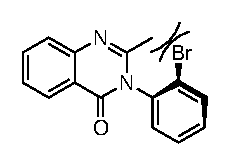
\includegraphics[scale=0.8]{Figures/mebroqualone.eps}
    \caption[The structure of mebroqualone.]{The structure of mebroqualone. Rotation is hindered about the biaryl bond, allowing the isolation of two atropisomers.}\label{fig:mebroqualone}
\end{figure}

\subsection{Biological systems}

\subsubsection{Proteins}
While we usually think of the tertiary structure of proteins as being dominated by H-bonding and hydrophobic effects, there is increasing evidence that Ch-bonding plays an important role as well.
This is not unexpected, as sulfur, a component of both cysteine and methionine, is known to form Ch-bonds in small molecules.
In the early days of Ch-bonding interactions (2001, before the name had come into common use) \citeauthor{Iwaoka2001} published an analysis of 604 protein structures in the Protein Data Bank (PDB).\autocite{Iwaoka2001}

A remarkable number of close contacts (sum of Van der Waals radii plus 0.5~\AA) between sulfur and Lewis basic (X) atoms were identified in the structures, with 33\% of cysteine residues and 22\% of methionine residues showing a close contact.
Furthermore, the geometric parameters of these contacts were studied, with more than half of all contacts having a \ce{S-S-X} (X = O, N) of 150--180\degree.
The observed contacts were ascribed to a $ \pi $(\ce{C=O}) $ \rightarrow \sigma^{\star} $(\ce{S-S}) interaction, in contrast to the n(X)$ \rightarrow \sigma^{\star} $(\ce{S-X}) interaction which dominates in small molecules.
Also contrary to the case of small molecules, the authors suggested that the orbital component of the interaction is small, though important for establishing the directionality of the interaction.
Dispersion appears to be the major stabilising force, as optimization using a non-dispersion corrected level of theory gave unrealistically large distances between the two interacting groups.

The differences between Ch-bonding in proteins and small molecules is likely due to variation in orbital energies in the functional groups which are found in each class.
While small molecule Ch-bond donors are characterised by easily accessible, low energy $ \sigma^{\star} $(\ce{Ch-X}) orbitals, these are simply not found in proteins.
Instead, donors are characterised by $ \sigma^{\star} $(\ce{S-S}) or $ \sigma^{\star} $(\ce{S-C}) orbitals, which are much higher in energy and less accessible to acceptors.
Ch-bond acceptors, too, are markedly different between small molecules and proteins.
In general, the HOMO of a system (the most Lewis basic site) is dominated by lone pairs.
This is observed in most small molecules, as they form Ch-bonds through these lone pairs.
However, the amide bond, which is ubiquitous in proteins, shows an unusual inversion in orbital energies.
The $ \pi $(\ce{C=O}) orbital is elevated with respect to the lone pair according to MP2 calculations, making it the more basic site.
Structural data supports this assertion, as the Ch-bond donor usually approaches the top of the C=O bond in proteins, rather than the usual approach towards the oxygen lone pair (\cref{fig:amide-diselenide-ch-bond}).\autocite{Iwaoka2012}

\begin{figure}
    \centering
    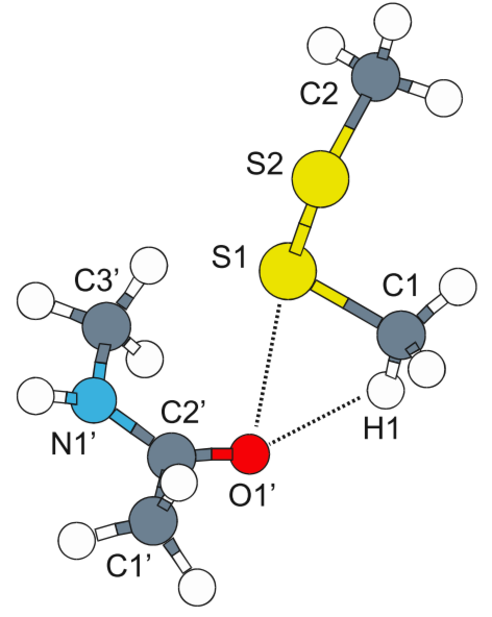
\includegraphics[width=0.4\linewidth]{Figures/amide-diselenide-ch-bond.pdf}
    \caption{Directional preference for Ch-bonded interactions in proteins.}\label{fig:amide-diselenide-ch-bond}
\end{figure}

It is worth noting that selenium is also found in proteins as selenocysteine and selenomethionine.
This would be expected to be an even stronger Ch-bond donor.
However, selenoproteins are relatively few in number, precluding such extensive statistical analysis.\autocite{Iwaoka2015}
They are only mentioned here for the sake of completeness.

Intramolecular interactions are just one instance of Ch-bonding in biological systems.
Proteins often interact with ligands or substrates through H-bonds, so it is reasonable to propose that Ch-bonding could be applied in this field as well.
Indeed, a protein-ligand Ch- and X-bonding interaction was used to target the gatekeeper methionine (MET146) residue of c-Jun N-terminal kinase 3 (JNK3) in a model study by \citeauthor{Lange2015}.\autocite{Lange2015}
In this work, a protein$ \rightarrow $ligand Ch-bond was used to stabilise the interaction.
Inhibition of a cysteine protease using a variety of sulfur-containing heterocyclic ligands was also investigated.\autocite{Giroud2017}
These ligands formed ligand$ \rightarrow $protein Ch-bonds, complementary to the the work by Lange.
Non-conventional protein-ligand interactions are summarised in a comprehensive review by \citeauthor{Beno2015}.\autocite{Beno2015}

\subsubsection{Nucleic acids}
Nucleic acids represent another application of Ch-bonding in biology.
In addition to their crucial role in the storage of genetic information, they have also been investigated as a structural material in nanotechnology.
The ubiquity of H-bonds in nucleic acid complexes suggests that $ \sigma $-hole interactions may also be used to direct formation of these complexes.
X-bonding was indeed able to be used to direct formation of a Holliday junction between two DNA strands (\cref{fig:holliday-junction}).\autocite{Voth2007}
Holliday junctions are branched nucleic acid structures that appear in many biological processes including recombination and double-strand break repair.
They are also useful as building blocks for DNA nanotechnology, where their self assembly and predictable geometry are exploited.
The authors estimated that the X-bonding interaction (mediated through a bromo-substituent) was 2--5 kcal/mol stronger than the corresponding H-bond.
A 2017 review identified a further 21 X-bonded nucleic acid structures.\autocite{Kolar2017}
X-bonding was in fact able to partially replace inter-strand H-bonding interaction in a DNA oligomer.\autocite{Parker2012}

\begin{figure}
    \centering
    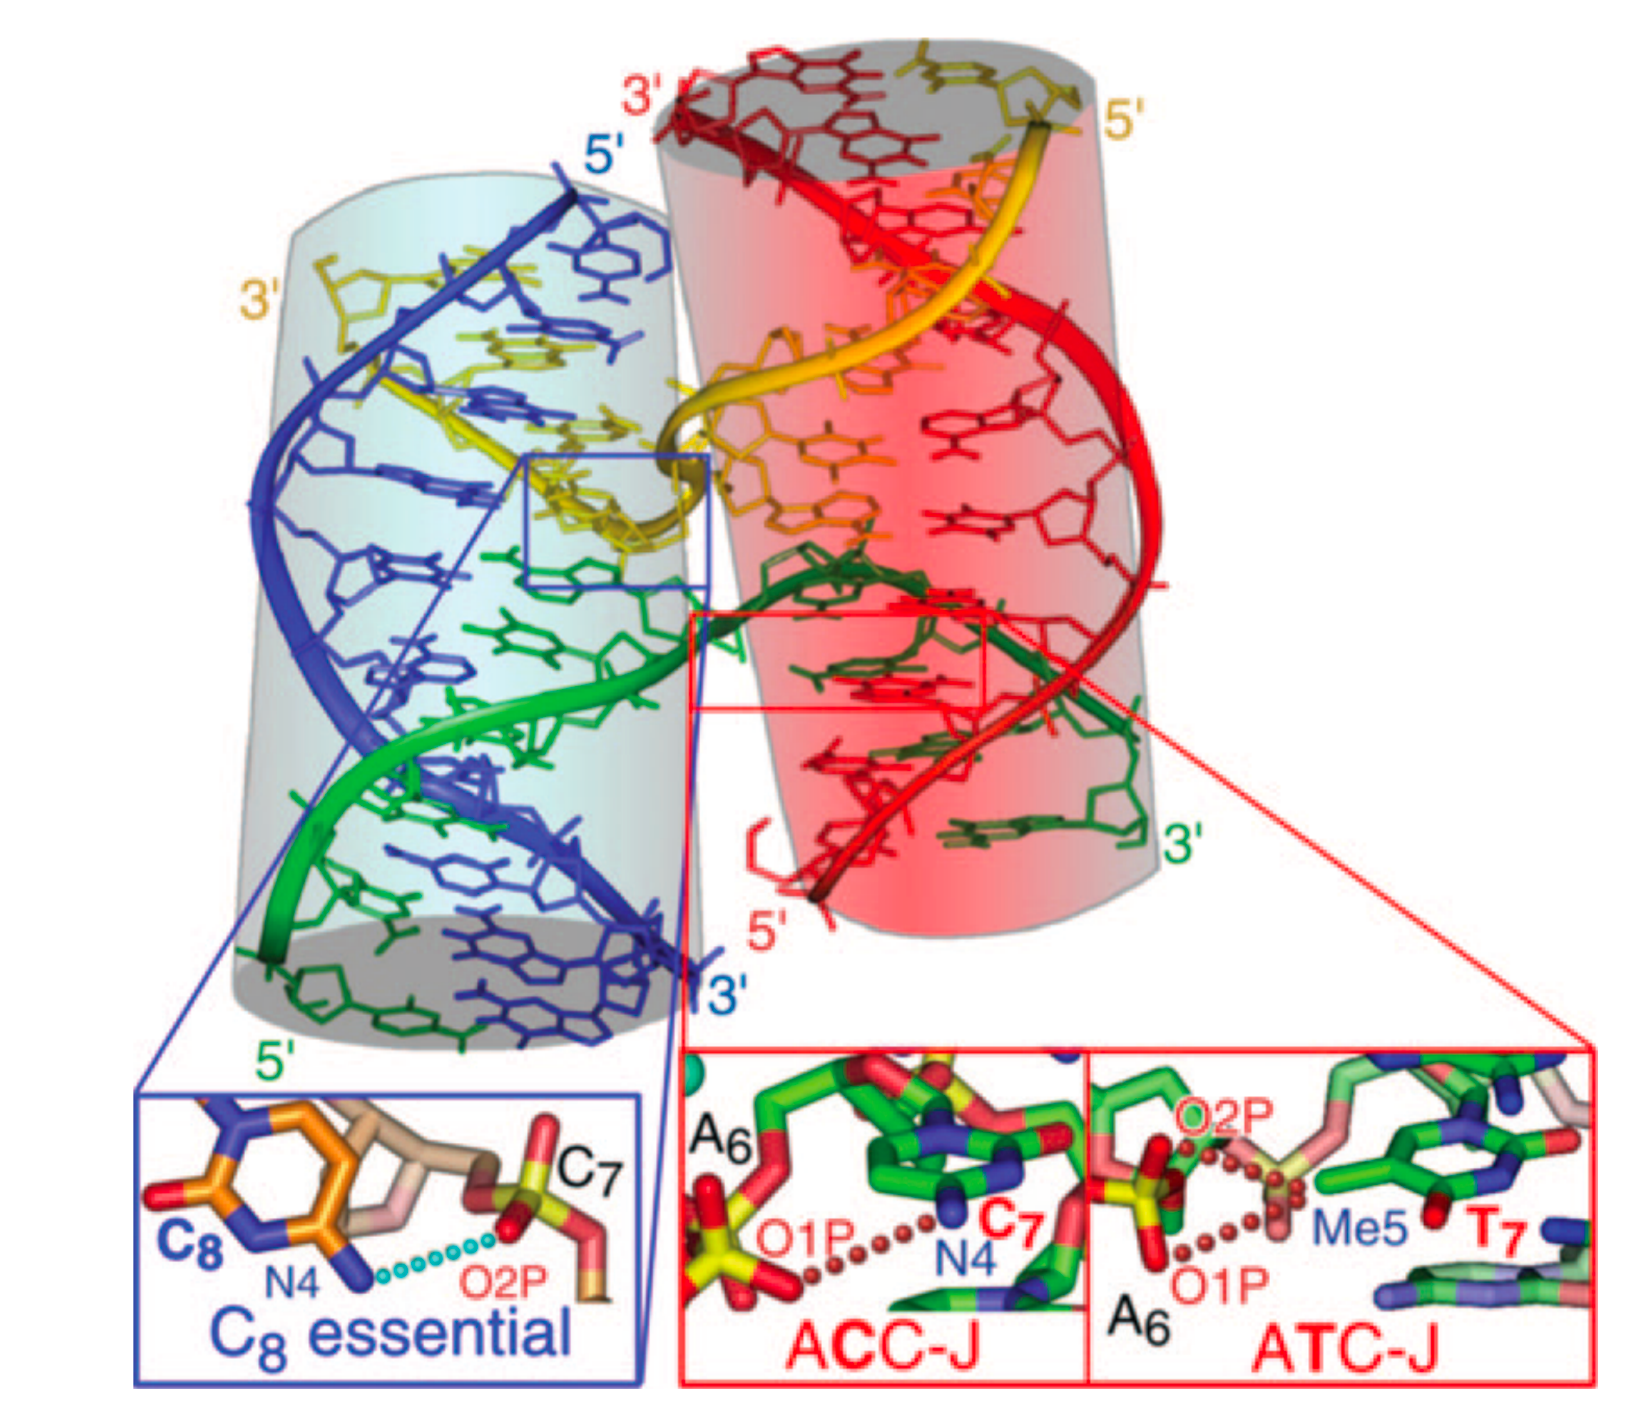
\includegraphics[width=0.6\linewidth]{Figures/holliday-junction.pdf}
    \caption{Holliday junction formed by X-bonding.\autocite{Voth2007}}\label{fig:holliday-junction}
\end{figure}

Ch-bonding, too, has been investigated in the context of nucleic acids.
\Citeauthor{Sharma2020} recently investigated the possibility of forming Ch-bonded analogues of the canonical A:T/G:C base pairs in order to expand the genetic alphabet.\autocite{Sharma2020}
A G\textsubscript{\ce{SeF}}:C dimer was found to be more stable than the canonical G:C pair, where the \ce{SeF} subscript indicates that one of the H-bond donors on the guanine was replaced by a selenenyl fluoride.
\Citeauthor{Farrell2018} showed that introducing heavy chalcogens into nucleobases has profound impacts on their photochemistry, with implications for their use in photodynamic therapy.\autocite{Farrell2018}
The photophysics of selenonucleobases has been further explored, showing that they are uniquely photo-stable while efficiently populating and depopulating their excited states.\autocite{Mai2019,Peng2020,Fang2019,Uleany2020}
While none of these investigations specifically mentioned Ch-bonding, it is highly likely that it would come into play, which may provide a means of directing the activity of these photo-sensitisers.

\begin{figure}
    \centering
    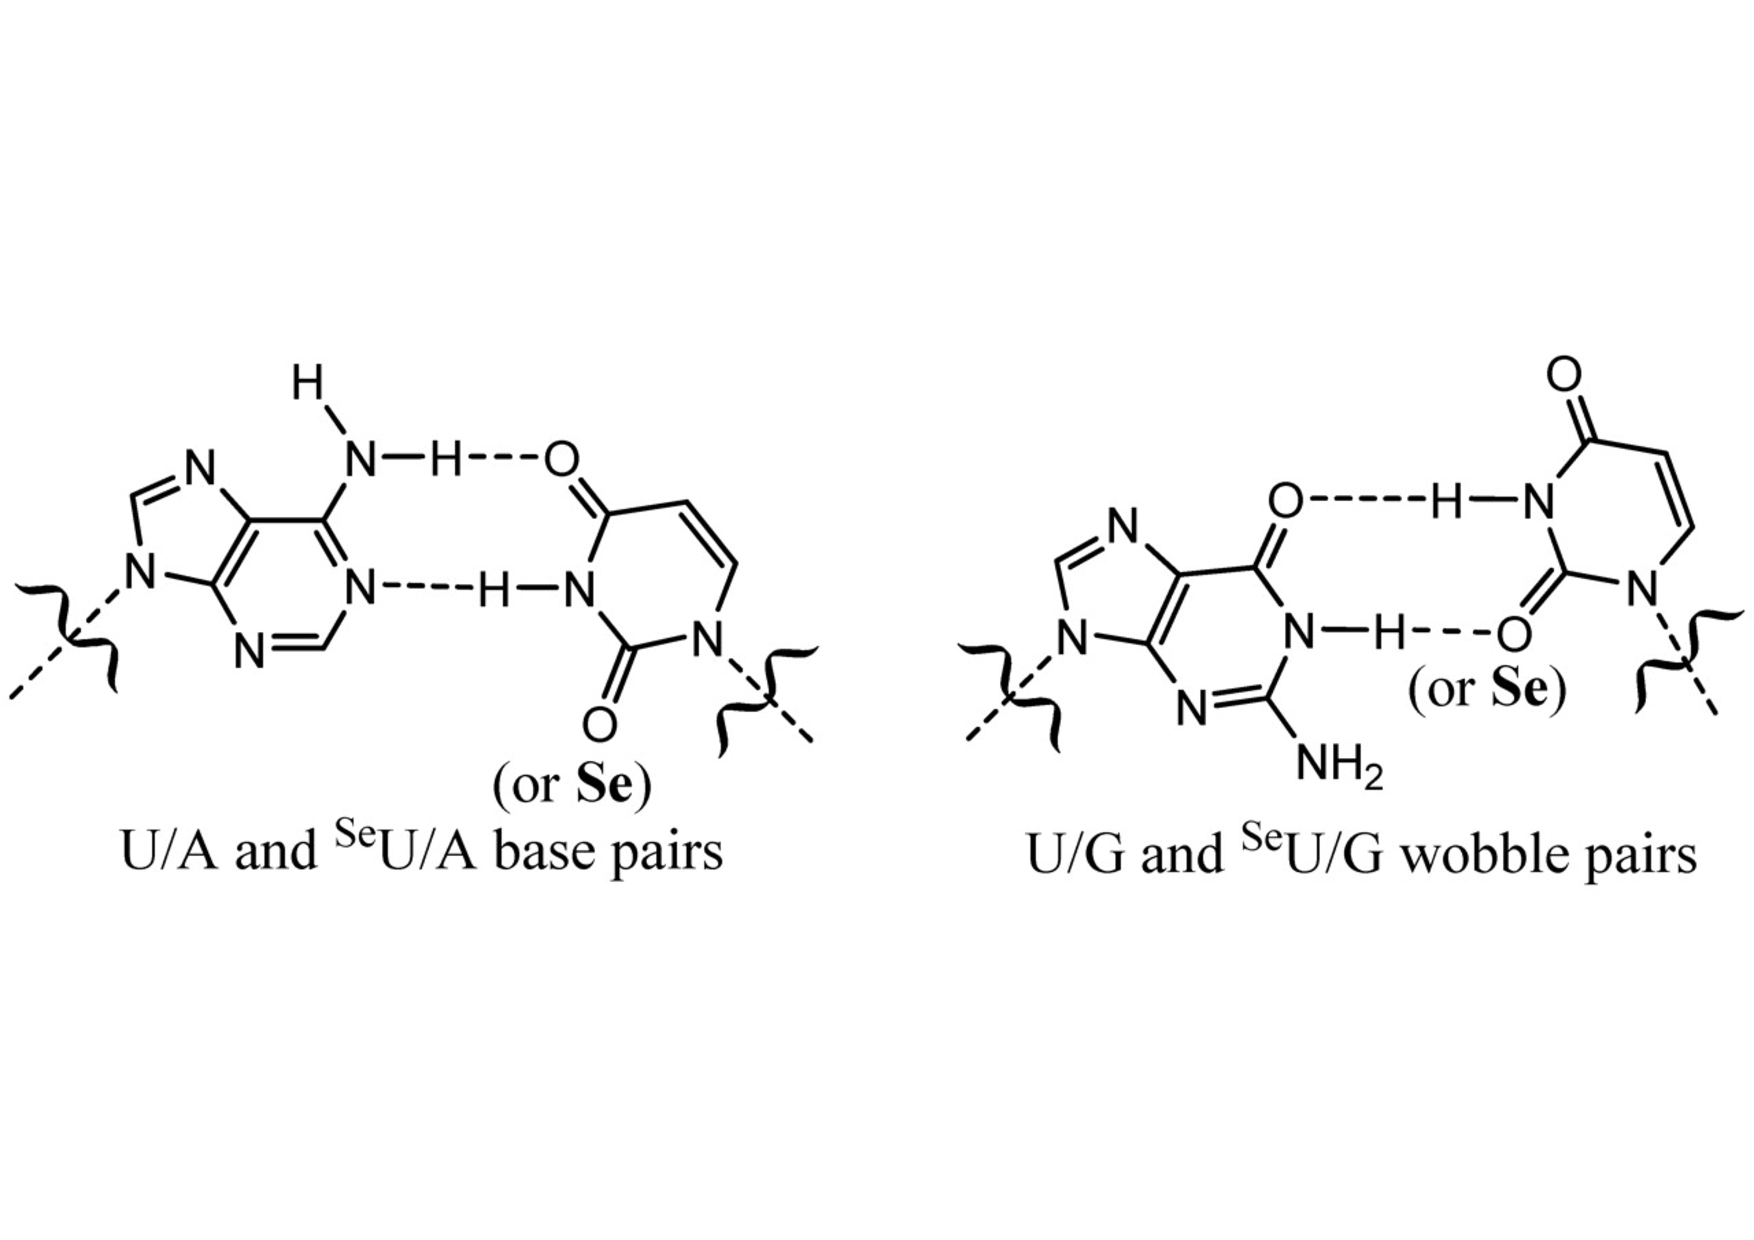
\includegraphics[width=0.6\linewidth]{Figures/wobble-bp.pdf}
    \caption[Canonical Watson-Crick U/A base pair, and the ``wobble'' U:G base pair in RNA.]{Canonical Watson-Crick U:A base pair, and the ``wobble'' U/G base pair in RNA.\@ The latter is disfavoured when an oxygen atom in uracil is substituted by selenium.}\label{fig:wobble-bp}
\end{figure}

Selenium has also been incorporated into nucleobases as a H-bond acceptor, in which it was shown that selenonucleobases can effectively discriminate against the formation of a so-called ``wobble'' base pair (U:G as opposed to U:A in RNA, or T:G/T:A in DNA, \cref{fig:wobble-bp}).\autocite{Hassan2010,Sun2012}
Another advantage of selenonucleobase incorporation is the ability to use the heavy selenium atom for MAD/SAD phasing of macromolecular crystal structures.\autocite{Salon2007}
This was also the motivation for a \citeyear{Conlon2019} study in which the selenium was incorporated into the phosphate backbone.\autocite{Conlon2019}
A major advantage of this approach is that the bulk of the selenium atom does not need to be accommodated in the interior of the double helix, so structural distortions are minimised.
To date, there have not been any drugs which target nucleic acids through Ch-bonding, which is an area we explore in \cref{ch:dna-binder}.

\section{Context of this work}
In this thesis, we examine some of the fundamental aspects of Ch-bonding in real-world systems, motivated by the end goal of developing a Ch-bonding DNA binder.
We identify the drug ebselen as a relevant molecule, and its benzisoselenazolinone core as a potent Ch-bond donor, and we begin with a crystallographic study of a series of co-crystals of ebselen derivatives and a variety of Lewis bases.
We show that benzisoselenazolinone derivatives reproducibly form Ch-bonded co-crystals, and extend this to a more comprehensive study in which the electronic properties of the donor are systematically varied.
Using this structural data, we show that there is a degree of covalency to Ch-bonding in these systems.
We also analyse the experimental electron density from high-quality diffraction measurements within the QTAIM framework (see \cref{sec:qtaim}), which suggests that these Ch-bonds are actually predominantly closed-shell in origin.
As part of our investigation into model Ch-bonded complexes, we use the unique NMR properties of the \ce{^{77}Se} nucleus to probe the electron density around the selenium atom, which shows promise as a method for characterising these compounds.

In a departure from selenium chemistry, we sought to answer the question of whether oxygen can act as a Ch-bond donor.
Preliminary computational studies suggested that highly reactive oxygen fluorides could act as Ch-bond donors\autocite{Varadwaj2019a}, but we demonstrate that an \textit{o}-nitro-O-aryl oxime displays characteristics consistent with an intramolecular \ce{O \cdots O} Ch-bond.
We prepare a number of analogues, and characterise the nature of the \ce{O \cdots O} interaction both crystallographically and computationally.
In a supplementary investigation, we manipulate the electronic properties of the Ch-bond donor and acceptor in a number of analogues, and show that the Ch-bond does indeed behave as one would expect.

Using the information from these fundamental studies into the nature of Ch-bonds, we prepare a Ch-bonding analogue of a Hoechst DNA binder and characterise its interaction with DNA.\@
An intermediate compound in this synthesis showed interesting crystal packing when recrystallised from different solvents.
Pyridine, a strong Lewis base, is incorporated into the crystal lattice in one dimensional channels, but is lost upon heating to around 80\degree{}C.
This loss is accompanied by a change in crystal packing and rearrangement of Ch-bonds, to the form which could be recrystallised from dimethylformamide.

Due to the global pandemic in 2020, lab work was unfeasible for a significant period.
During this time, we turned to studying Ch-bonding computationally.
Early on in the pandemic, ebselen was identified as an inhibitor of the SARS-CoV2 M\textsuperscript{pro} main protease, which plays a crucial role in viral replication.\autocite{Jin2020}
In light of this, there were a number of computational studies in which ebselen was ``docked'' to the protein target using a molecular mechanics force field.
However, typical force fields are not able to describe Ch-bonding, which we (and others) had identified as central to the chemistry of ebselen.
We therefore developed an extension of the General Amber Force Field (GAFF) which models Ch-bonding by including a positively charged pseudoatom, which can form directional, stabilising interactions, similar to Ch-bonds.
We used this force field to model a number of the complexes we had previously studied crystallographically, and also validated the approach by modelling the encounter complex formed between ebselen and SOD1, a known target.

% short summary?

\printbibliography[heading=subbibliography]
\end{refsection}
